\documentclass{ximera}

\usepackage{todonotes}

\newcommand{\RR}{\mathbb R}
\renewcommand{\d}{\,d}
\newcommand{\dd}[2][]{\frac{d #1}{d #2}}
\renewcommand{\l}{\ell}
\newcommand{\ddx}{\frac{d}{dx}}
\newcommand{\dfn}{\textbf}
\newcommand{\eval}[1]{\bigg[ #1 \bigg]}
\renewcommand{\epsilon}{\varepsilon}
\newcommand{\p}[1]{\left(#1\right)}
\newcommand{\br}[1]{\left[#1\right]}
\newcommand{\set}[1]{\left\{#1\right\}}


\let\prelim\lim
\renewcommand{\lim}{\displaystyle\prelim}

\colorlet{textColor}{black} 
\colorlet{background}{white}
\colorlet{penColor}{blue!50!black} % Color of a curve in a plot
\colorlet{penColor2}{red!50!black}% Color of a curve in a plot
\colorlet{penColor3}{red!50!blue} % Color of a curve in a plot
\colorlet{penColor4}{green!50!black} % Color of a curve in a plot
\colorlet{penColor5}{orange!80!black} % Color of a curve in a plot
\colorlet{fill1}{blue!50!black!20} % Color of fill in a plot
\colorlet{fill2}{blue!10} % Color of fill in a plot
\colorlet{fillp}{fill1} % Color of positive area
\colorlet{filln}{red!50!black!20} % Color of negative area
\colorlet{gridColor}{gray!50} % Color of grid in a plot


\newcommand{\fullwidth}{}
\newcommand{\normalwidth}{}



%% makes a snazzy t-chart for evaluating functions
\newenvironment{tchart}{\rowcolors{2}{}{background!90!textColor}\array}{\endarray}


\author{Gregory Hartman \and Matthew Carr}
\license{Creative Commons 3.0 By-NC}
\acknowledgement{https://github.com/APEXCalculus}

\begin{document}

\begin{exercise}

\outcome{Calculate limits using the limit laws.}
\outcome{Calculate limits of the form 0/0.}

\tag{limit}
\tag{discontinuous}
\tag{indeterminate form}

  Find 
  \[
  \lim_{x\to-1}\p{ \frac{x^2+8x+7}{x^2+6x+5}}
  \begin{prompt}
  = \answer{1.5}.
  \end{prompt}
  \]
    \begin{hint}
      This function is \underline{not} continuous everywhere, but both the numerator and denominator are continuous everywhere as functions. Thus, if the limit of $\frac{x^2+8x+7}{x^2+6x+5}$ as $x\to{a}$ does not exist, then the denominator $x^2+6x+5$ must be zero at $a$. Does $x^2+6x+5=0$ when $x=-1$? Does $x^2+8x+7=0$ at $x=-1$ as well?
    \end{hint}
     \begin{hint}
    Take a look at the graph of the function
    \begin{center}
     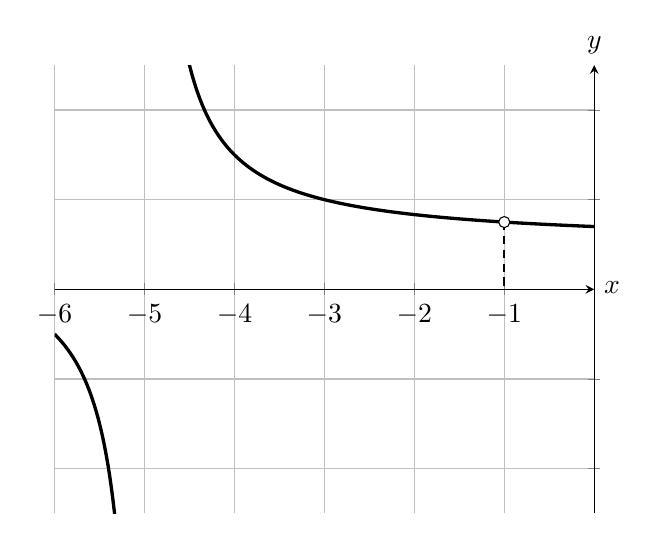
\begin{tikzpicture}
	\begin{axis}
	[ymin=-5,ymax=5, axis lines=center,xlabel=$x$,ylabel=$y$,every axis y 
	label/.style={at=(current axis.above origin),anchor=south},every axis x label/.style={at=(current axis.right of origin),anchor=west},
	domain=-6:0,
	yticklabels={},
	ymajorgrids=true,
	grid = major
	]
	\addplot[domain=-6:-501/100,very thick,smooth,samples=600]
	{(\x^2+8*\x+7)/(\x^2+6*\x+5)};
	\addplot[domain=-499/100:0,very thick,smooth,samples=600]
	{(\x^2+8*\x+7)/(\x^2+6*\x+5)};
	\draw[densely dashed, thick] (axis cs:-1,1.5)--(axis cs:-1,0);
	\draw[fill=white] (axis cs:-1,1.5) circle [radius=2pt];
	\end{axis}
       \end{tikzpicture}      
      \end{center}
      There is a removable discontinuity at $x=-1$. This suggests something about the factorization of both polynomials $x^2+8x+7$ and $x^2+6x+5$. Recall that if both $\lim_{x\to a}f\p{x}$ and $\lim_{x\to a}g\p{x}$ exist, then, if $\lim_{x\to a}g\p{x}\ne0$, then $\lim_{x\to a}\frac{f\p{x}}{g\p{x}}=\frac{\lim_{x\to a}f\p{x}}{\lim_{x\to a}g\p{x}}$.
    \end{hint}
    \begin{hint}
     Notice that the quadratic equation tells us that $x^2+8x+7=0$ has solutions $-4\pm3$ and $x^2+6x+5=0$ has solutions $-3\pm{2}$. Thus, $x^2+8x+7=\left(x+1\right)\left(x+7\right)$ and $x^2+6x+5=\left(x+1\right)\left(x+5\right)$. Then for all $x\ne-1$, $\frac{x^2+8x+7}{x^2+6x+5}=\frac{x+7}{x+5}$, upon canceling the common factor of $\p{x+1}$. Since we are not asking what value $\frac{x^2+8x+7}{x^2+6x+5}$ takes at $x=-1$, but rather what value $\frac{x^2+8x+7}{x^2+6x+5}$ \underline{approaches} as $x\to-1$, it suffices in every case to look at $\lim_{x\to-1}\p{\frac{x+7}{x+5}}$. We see that $\lim_{x\to-1}\p{x+7}=6$ while $\lim_{x\to-1}\p{x+5}=4$, and since $\lim_{x\to-1}\p{x+5}\ne0$, $\lim_{x\to-1}\p{\frac{x+7}{x+5}}=\frac{\lim_{x\to-1}\p{x+7}}{\lim_{x\to-1}\p{x+5}}=\frac{3}{2}$. Or, in decimal form, $1.5$.
    \end{hint}
\end{exercise}

\end{document}